
\documentclass[letterpaper,hide notes,xcolor={table,svgnames},pdftex,10pt]{beamer}
\def\showexamples{t}

\usecolortheme{crane}
\setbeamertemplate{navigation symbols}{}

\usetheme{MyPittsburgh}
\usepackage{hyperref}
\usepackage{graphicx,xspace}
\usepackage[normalem]{ulem}
\usepackage{multicol}
\usepackage{amsmath,amssymb,amsthm,graphicx,xspace}
\newcommand\SF[1]{$\bigstar$\footnote{SF: #1}}

\usepackage[sfdefault,lf]{carlito}
\usepackage[T1]{fontenc}
\usepackage[scaled]{beramono}
\usepackage{tikzpagenodes}
\newcommand{\Rplus}{\protect\hspace{-.1em}\protect\raisebox{.35ex}{\small{\small\textbf{+}}}}
\newcommand{\Cpp}{\mbox{C\Rplus\Rplus}\xspace}

\newcounter{tmpnumSlide}
\newcounter{tmpnumNote}

\newcommand\mnote[1]{%
	\addtocounter{tmpnumSlide}{1}
	\ifdefined\showcues {~\tiny\fbox{\arabic{tmpnumSlide}}}\fi
	\note{\setlength{\parskip}{1ex}\addtocounter{tmpnumNote}{1}\textbf{\Large \arabic{tmpnumNote}:} {#1\par}}}

\newcommand\mmnote[1]{\note{\setlength{\parskip}{1ex}#1\par}}


\newcommand\mquestion[2]{{~\color{red}\fbox{?}}\note{\setlength{\parskip}{1ex}\par{\Large \textbf{?}} #1} \note{\setlength{\parskip}{1ex}\par{\Large \textbf{A}} #2\par}\ifdefined \presentationonly \pause \fi}

\newcommand\blackboard[1]{%
	\ifdefined   \showblackboard
		{#1}
	\else {\begin{center} \fbox{\colorbox{blue!30}{%
						\begin{minipage}{.95\linewidth}%
							\hspace{\stretch{1}} Some space intentionally left blank; done at the blackboard.%
						\end{minipage}}}\end{center}}%
	\fi%
}

\usepackage{listings}
\lstset{%
	keywordstyle=\bfseries,
	aboveskip=15pt,
	belowskip=15pt,
	captionpos=b,
	identifierstyle=\ttfamily,
	frame=lines,
	numbers=left, basicstyle=\scriptsize, numberstyle=\tiny, stepnumber=0, numbersep=2pt}

\usepackage{siunitx}
\newcommand\sius[1]{\num[group-separator = {,}]{#1}\si{\micro\second}}
\newcommand\sims[1]{\num[group-separator = {,}]{#1}\si{\milli\second}}
\newcommand\sins[1]{\num[group-separator = {,}]{#1}\si{\nano\second}}
\sisetup{group-separator = {,}, group-digits = true}

%% -------------------- tikz --------------------
\usepackage{tikz}
\usetikzlibrary{positioning}
\usetikzlibrary{arrows,backgrounds,automata,decorations.shapes,decorations.pathmorphing,decorations.markings,decorations.text}

\tikzstyle{place}=[circle,draw=blue!50,fill=blue!20,thick, inner sep=0pt,minimum size=6mm]
\tikzstyle{transition}=[rectangle,draw=black!50,fill=black!20,thick, inner sep=0pt,minimum size=4mm]

\tikzstyle{block}=[rectangle,draw=black, thick, inner sep=5pt]
\tikzstyle{bullet}=[circle,draw=black, fill=black, thin, inner sep=2pt]

\tikzstyle{pre}=[<-,shorten <=1pt,>=stealth',semithick]
\tikzstyle{post}=[->,shorten >=1pt,>=stealth',semithick]
\tikzstyle{bi}=[<->,shorten >=1pt,shorten <=1pt, >=stealth',semithick]

\tikzstyle{mut}=[-,>=stealth',semithick]

\tikzstyle{treereset}=[dashed,->, shorten >=1pt,>=stealth',thin]

\usepackage{ifmtarg}
\usepackage{xifthen}
\makeatletter
% new counter to now which frame it is within the sequence
\newcounter{multiframecounter}
% initialize buffer for previously used frame title
\gdef\lastframetitle{\textit{undefined}}
% new environment for a multi-frame
\newenvironment{multiframe}[1][]{%
	\ifthenelse{\isempty{#1}}{%
		% if no frame title was set via optional parameter,
		% only increase sequence counter by 1
		\addtocounter{multiframecounter}{1}%
	}{%
		% new frame title has been provided, thus
		% reset sequence counter to 1 and buffer frame title for later use
		\setcounter{multiframecounter}{1}%
		\gdef\lastframetitle{#1}%
	}%
	% start conventional frame environment and
	% automatically set frame title followed by sequence counter
	\begin{frame}%
		\frametitle{\lastframetitle~{\normalfont(\arabic{multiframecounter})}}%
		}{%
	\end{frame}%
}
\makeatother

\makeatletter
\newdimen\tu@tmpa%
\newdimen\ydiffl%
\newdimen\xdiffl%
\newcommand\ydiff[2]{%
	\coordinate (tmpnamea) at (#1);%
	\coordinate (tmpnameb) at (#2);%
	\pgfextracty{\tu@tmpa}{\pgfpointanchor{tmpnamea}{center}}%
	\pgfextracty{\ydiffl}{\pgfpointanchor{tmpnameb}{center}}%
	\advance\ydiffl by -\tu@tmpa%
}
\newcommand\xdiff[2]{%
	\coordinate (tmpnamea) at (#1);%
	\coordinate (tmpnameb) at (#2);%
	\pgfextractx{\tu@tmpa}{\pgfpointanchor{tmpnamea}{center}}%
	\pgfextractx{\xdiffl}{\pgfpointanchor{tmpnameb}{center}}%
	\advance\xdiffl by -\tu@tmpa%
}
\makeatother
\newcommand{\copyrightbox}[3][r]{%
	\begin{tikzpicture}%
		\node[inner sep=0pt,minimum size=2em](ciimage){#2};
		\usefont{OT1}{phv}{n}{n}\fontsize{4}{4}\selectfont
		\ydiff{ciimage.south}{ciimage.north}
		\xdiff{ciimage.west}{ciimage.east}
		\ifthenelse{\equal{#1}{r}}{%
			\node[inner sep=0pt,right=1ex of ciimage.south east,anchor=north west,rotate=90]%
			{\raggedleft\color{black!50}\parbox{\the\ydiffl}{\raggedright{}#3}};%
		}{%
			\ifthenelse{\equal{#1}{l}}{%
				\node[inner sep=0pt,right=1ex of ciimage.south west,anchor=south west,rotate=90]%
				{\raggedleft\color{black!50}\parbox{\the\ydiffl}{\raggedright{}#3}};%
			}{%
				\node[inner sep=0pt,below=1ex of ciimage.south west,anchor=north west]%
				{\raggedleft\color{black!50}\parbox{\the\xdiffl}{\raggedright{}#3}};%
			}
		}
	\end{tikzpicture}
}


%% --------------------

%\usepackage[excludeor]{everyhook}
%\PushPreHook{par}{\setbox0=\lastbox\llap{MUH}}\box0}

%\vspace*{\stretch{1}

%\setbox0=\lastbox \llap{\textbullet\enskip}\box0}

\setlength{\parskip}{\fill}

\newcommand\noskips{\setlength{\parskip}{1ex}}
\newcommand\doskips{\setlength{\parskip}{\fill}}

\newcommand\xx{\par\vspace*{\stretch{1}}\par}
\newcommand\xxs{\par\vspace*{2ex}\par}
\newcommand\tuple[1]{\langle #1 \rangle}
\newcommand\code[1]{{\sf \footnotesize #1}}
\newcommand\ex[1]{\uline{Example:} \ifdefined \presentationonly \pause \fi
	\ifdefined\showexamples#1\xspace\else{\uline{\hspace*{2cm}}}\fi}

\newcommand\ceil[1]{\lceil #1 \rceil}


\AtBeginSection[]
{
	\begin{frame}
		\frametitle{Outline}
		\tableofcontents[currentsection]
	\end{frame}
}



\pgfdeclarelayer{edgelayer}
\pgfdeclarelayer{nodelayer}
\pgfsetlayers{edgelayer,nodelayer,main}

\tikzstyle{none}=[inner sep=0pt]
\tikzstyle{rn}=[circle,fill=Red,draw=Black,line width=0.8 pt]
\tikzstyle{gn}=[circle,fill=Lime,draw=Black,line width=0.8 pt]
\tikzstyle{yn}=[circle,fill=Yellow,draw=Black,line width=0.8 pt]
\tikzstyle{empty}=[circle,fill=White,draw=Black]
\tikzstyle{bw} = [rectangle, draw, fill=blue!20,
text width=4em, text centered, rounded corners, minimum height=2em]

\newcommand{\CcNote}[1]{% longname
	This work is licensed under the \textit{Creative Commons #1 3.0 License}.%
}
\newcommand{\CcImageBy}[1]{%
	\includegraphics[scale=#1]{creative_commons/cc_by_30.pdf}%
}
\newcommand{\CcImageSa}[1]{%
	\includegraphics[scale=#1]{creative_commons/cc_sa_30.pdf}%
}
\newcommand{\CcImageNc}[1]{%
	\includegraphics[scale=#1]{creative_commons/cc_nc_30.pdf}%
}
\newcommand{\CcGroupBySa}[2]{% zoom, gap
	\CcImageBy{#1}\hspace*{#2}\CcImageNc{#1}\hspace*{#2}\CcImageSa{#1}%
}
\newcommand{\CcLongnameByNcSa}{Attribution-NonCommercial-ShareAlike}

\newenvironment{changemargin}[1]{% 
	\begin{list}{}{% 
		\setlength{\topsep}{0pt}% 
		\setlength{\leftmargin}{#1}% 
		\setlength{\rightmargin}{1em}
		\setlength{\listparindent}{\parindent}% 
		\setlength{\itemindent}{\parindent}% 
		      \setlength{\parsep}{\parskip}% 
		      }% 
		\item[]}{\end{list}}




\title{Lecture 20 --- Memory }

\author{Jeff Zarnett \\ \small \texttt{jzarnett@uwaterloo.ca}}
\institute{Department of Electrical and Computer Engineering \\
  University of Waterloo}
\date{\today}


\begin{document}

\begin{frame}
  \titlepage

 \end{frame}


\begin{frame}
\frametitle{Main Memory}

\begin{center}
	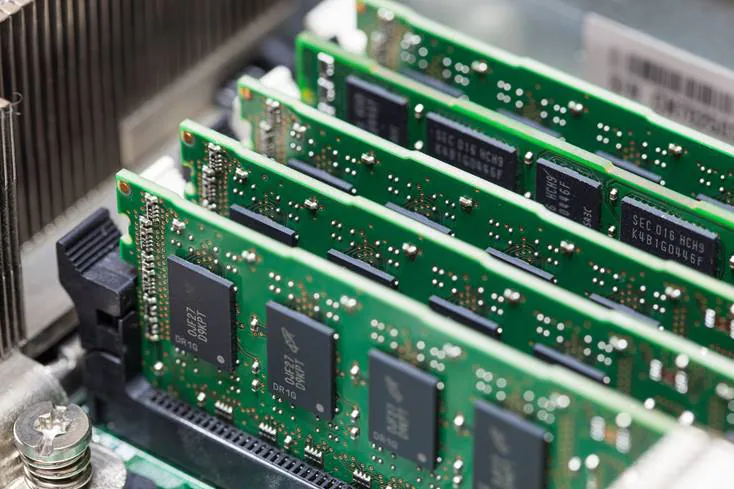
\includegraphics[width=0.65\textwidth]{images/ram.jpg}
\end{center}

Fetch instructions from memory, fetch operands, write result.

... All to or from memory!

 \end{frame}


\begin{frame}
\frametitle{Main Memory}

\begin{center}
	
\includegraphics[width=0.5\textwidth]{images/waiting-for-the-bus.jpg}
\end{center}

A single simple instruction like an addition could result in 4 memory accesses. 

Therefore, we are spending a lot of time interacting with memory.


\end{frame}

\begin{frame}
\frametitle{Memory as a Resource}

Application developers behave as if:\\
\quad (1) main memory is unlimited; and \\
\quad (2) all of main memory is at the program's disposal. 


Why do program developers pretend that memory is infinite and unshared?

\end{frame}

\begin{frame}
\frametitle{Size Matters Not}

Compared to the early days of computing, memory available is huge. 

\begin{center}
	
\includegraphics[width=0.5\textwidth]{images/yoda.jpg}
\end{center}


The Commodore~64, introduced in 1982, had a whopping 64~KB of memory. 

A 4-byte (32-bit) integer was a significant fraction of memory. 

\end{frame}

\begin{frame}
\frametitle{Size Matters Not}

Application developers had to scrimp and save to avoid wasting even a single integer's worth of memory. 

This is why languages like C and Java support types like \texttt{short}.

\begin{center}
	
\includegraphics[width=0.4\textwidth]{images/pennypincher.jpg}
\end{center}

\end{frame}

\begin{frame}
\frametitle{Size Matters Not}

Now: if 1000 integers were wasted unnecessarily, would anyone notice or care?

``Kicking the can down the road''

Even though memory might be big enough for every process to have its own area, that would not work if every developer assumes memory is unshared. 


\end{frame}

\begin{frame}
\frametitle{The OS as Manager}

Modern operating systems manage the shared resource of memory for them. 

This was not always the case; applications used to be responsible for it.

There were third party programs to let the user do some, too. 


\end{frame}


\begin{frame}
\frametitle{The Empire is on the Verge of Success}

\begin{center}
	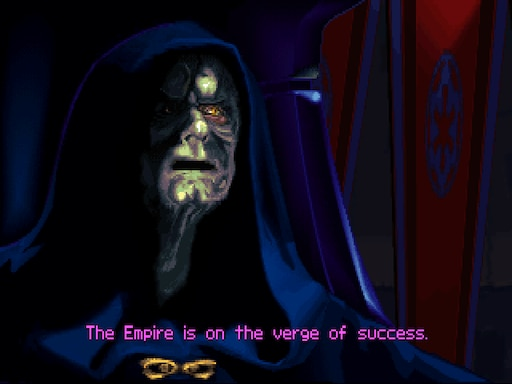
\includegraphics[width=0.7\textwidth]{images/empire-success.jpg}
\end{center}


\url{https://www.youtube.com/watch?v=KMFycV3SS9o}


\end{frame}

\begin{frame}
\frametitle{No Memory Management}

The simplest way to manage memory is, well, not to manage memory at all.

Early mainframe computers and even personal computers into the 1980s had no memory management strategy. 

Programs would just operate directly on memory addresses. 

\end{frame}

\begin{frame}
\frametitle{No Memory Management}

The section of memory that is program-accessible depended a lot on the operating system, if any, and other things needed (e.g., the BASIC compiler). 

So to write a program, we need to know the ``start'' \& ``end'' address. 


These would differ from machine to machine, making it that much harder to write a program that ran on different computers.



\end{frame}

\begin{frame}
\frametitle{No Memory Management - No Rules}

A program executed an instruction directly on a memory address, such as writing 385 into memory location 1024. 

Suppose you wanted to have two programs running at the same time. 

\begin{center}
	
\includegraphics[width=0.3\textwidth]{images/chaos.jpg}
\end{center}

If the first program writes to address 1024, and the second program writes to address 1024, the second program overwrote the first program's changes. 

\end{frame}

\begin{frame}
\frametitle{No Memory Management - No Rules}

Alternatively, the first program can use memory locations less than, say, 2048 and the second uses memory locations above 2048. 

This level of co-ordination gets more and more difficult as more and more programs are introduced to the system.

It is next to impossible if we do not control (have the source code to) all the programs that are to execute concurrently.



\end{frame}

\begin{frame}
\frametitle{No Memory Management - A Solution}

On every process switch, save the entire contents of memory to disk.\\
\quad Then restore the memory contents of the next process to run. 

This kind of swapping is, to say the least, incredibly expensive.

But the problem is avoided; only 1 process is ever in memory at a time.


\end{frame}

\begin{frame}
\frametitle{Jumping without a Parachute}

Another problem: there is no protection for the operating system. 

\begin{center}
	
\includegraphics[width=0.7\textwidth]{images/wileecoyote.jpg}
\end{center}

\end{frame}

\begin{frame}
\frametitle{Jumping without a Parachute}

The operating system is typically placed in either low memory or high memory, or in some cases, a bit of both. 

An errant memory access might overwrite a part of the OS in memory.

This can not only lead to crashes, but also corrupting important files on disk.



\end{frame}

\begin{frame}
\frametitle{IBM 360 Solution}

 The IBM 360 solved this problem by dividing memory into 2~KB blocks and each was assigned a 4-bit protection key, held in special registers in the CPU. 
 
The Program Status Word (PSW) also contained a 4 bit key. 

The 360 hardware would then identify as an error an attempt to access memory with a protection code different from the PSW key. 

The OS was the only software allowed to change the protection keys. 

Thus, no program could interfere with another or with the operating system


\end{frame}

\begin{frame}
\frametitle{Base and Limit}

We can generalize this solution by having two values maintained: 

The \alert{base} and \alert{limit} addresses. 

These define the start and end addresses of the program's memory.

Every memory access is compared to the base and the [base + limit] address. 

If an attempted memory access falls outside that acceptable range: error. 

\end{frame}

\begin{frame}
\frametitle{Base and Limit}

The base \& limit variables are often registers; comparison is done via hardware.

\begin{center}
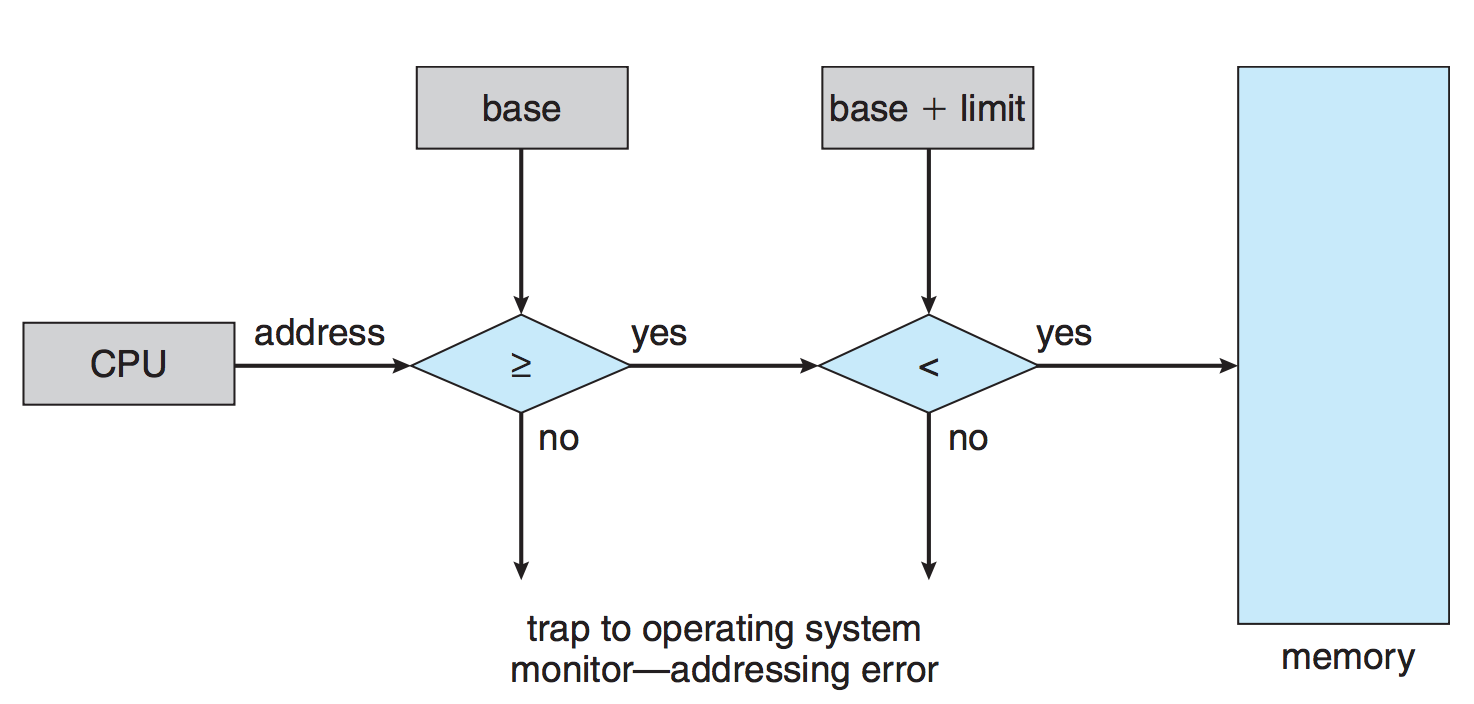
\includegraphics[width=0.9\textwidth]{images/memory-baselimit.png}
\end{center}


\end{frame}

\begin{frame}
\frametitle{Base and Limit}

Imagine we have two programs numbers simply 1 and 2, each 16~KB in size.

We will load them into memory in different consecutive areas:

\begin{center}
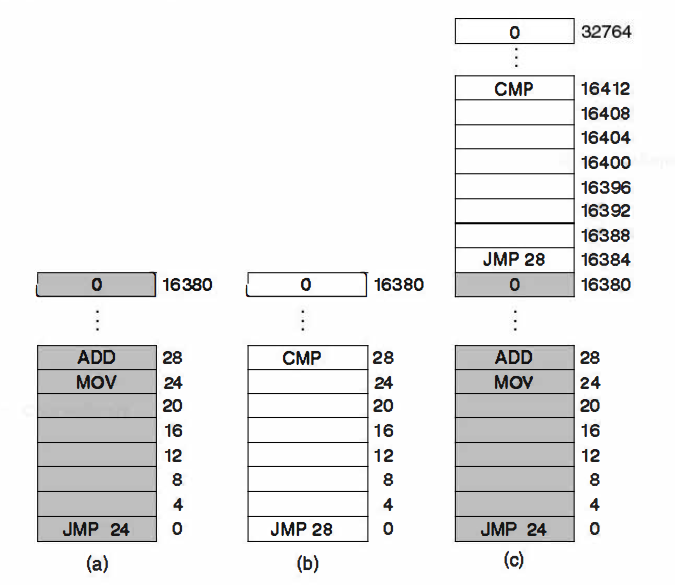
\includegraphics[width=0.70\textwidth]{images/os360.png}
\end{center}


\end{frame}

\begin{frame}
\frametitle{Base and Limit Problem}

Program 1 will execute as expected. 

The problem is immediately obvious when Program 2 runs. 

The instruction at address 16384 is executed: \texttt{JMP 28} takes execution to memory address 28 and not the expected address of 16412. 

The problem is that both programs reference absolute physical locations. 

\end{frame}

\begin{frame}
\frametitle{Static Relocation}

The IBM 360's stopgap solution to this was to do static relocation.

If a program was being loaded to a base address 16384 the constant 16384 was added to every program address during the load process. 

While slow, if every address is updated correctly, the program works.



\end{frame}

\begin{frame}
\frametitle{Static Relocation is Hard}

A command like \texttt{JMP 28} must be relocated, but the 28 in a command like \texttt{ADD~R1,28} is a constant and should not be changed. 

How do we know which is an address and which is a constant? 

It gets worse: in C a pointer contains an address, but addresses are just numbers. 

So in theory we could just dereference any integer variable and it would take us to a memory address (whether it's valid or not is not the point here). 

That makes it even harder to know if a number is just a number or an address.


\end{frame}

\begin{frame}
\frametitle{Variable Names}

When we are writing a program, unless it's in assembly, we do not usually refer to variables by their memory locations.

The command we write looks something like \texttt{x = 5;} 

We know that variable \texttt{x} is stored in memory, the question arises: when is the variable assigned a location in memory?


\end{frame}

\begin{frame}
\frametitle{Assigning a Variable a Location}

There are three opportunities to assign a variable a place in memory:

\begin{enumerate}
	\item \textbf{Compile time}
	\item \textbf{Load time}
	\item \textbf{Execution time}
\end{enumerate}


\end{frame}

\begin{frame}
\frametitle{Address Space}

It is clear that having no memory management leaves us with a number of problems. 

We need an abstraction; a layer of indirection. 

We do this with a concept called \alert{address space}. 


\end{frame}

\begin{frame}
\frametitle{Address Space}

An address space is a set of addresses that a process can use.

Each process has its own address space, independent of other processes'.\\
\quad Except when we create shared memory.

\end{frame}



\begin{frame}
\frametitle{Address Space: Telephone Numbers}
Telephone numbers in Canada and the USA take the form of NNN-NNNN.

In theory, any number in the range 000-0000 to 999-9999 could be issued, but in practice certain numbers are reserved (like the 000 or 555 prefixes).

Given the number of phones in the countries, 7 digits can't possibly be enough.

\end{frame}

\begin{frame}
\frametitle{Address Space: Telephone Numbers}

\begin{center}
	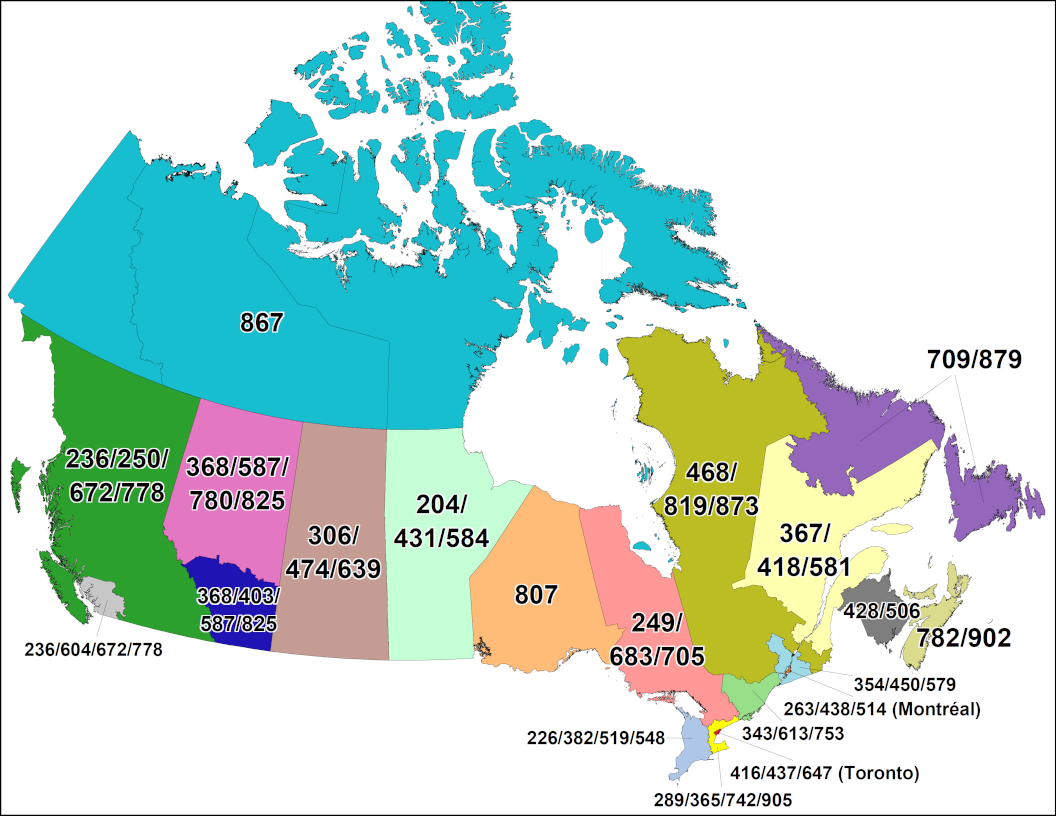
\includegraphics[width=0.9\textwidth]{images/areacodes.png}
\end{center}

\end{frame}

\begin{frame}
\frametitle{Area Codes for Memory}

This is the idea we want to apply: let each process have its own area code. 

So process can write to location 1024 and process 2 can write to location 1024 and these are two distinct locations, perhaps 21024 and 91024 respectively.

Now, instead of altering the addresses in memory, we will effectively prefix every memory access with an area code.

\end{frame}

\begin{frame}
\frametitle{Area Codes for Memory}

The address that is generated by the CPU, e.g., the 28 in \texttt{JMP 28}, is the \alert{logical address}. 

We then add the area code to it to produce the \alert{physical address} (the actual location in memory and the address that it sent over the bus). 


\end{frame}

\begin{frame}
\frametitle{Relocation Register}

In practice, to speed this up, it is done via some hardware, and the ``area code'' is a register called the \alert{relocation register}:

\begin{center}
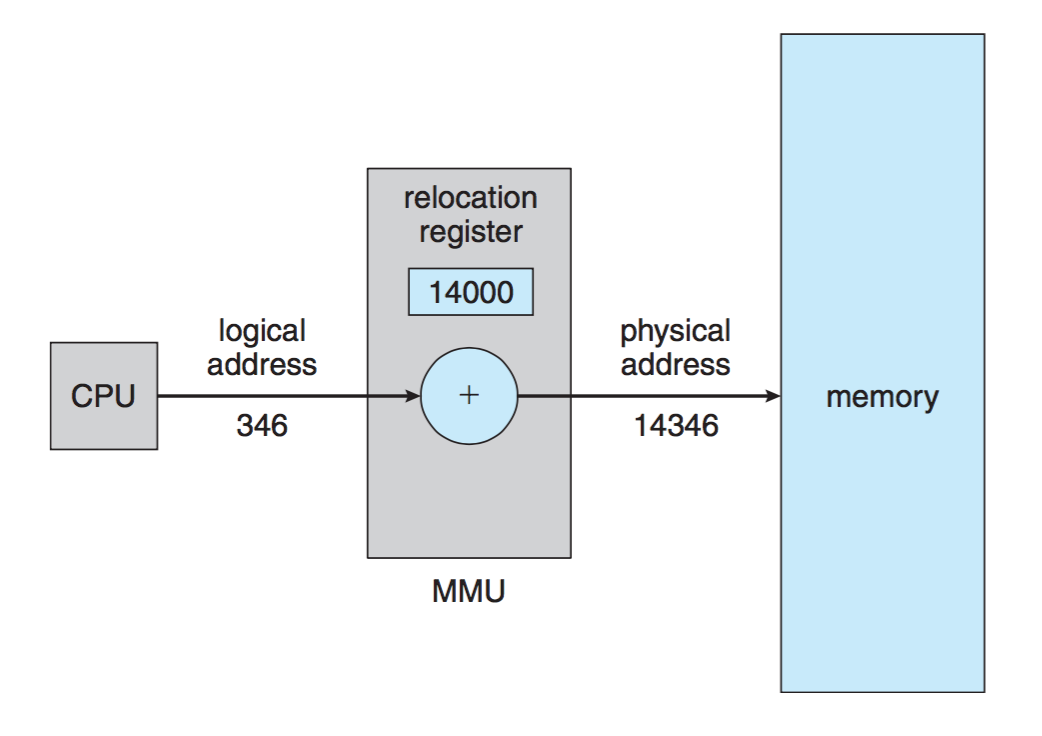
\includegraphics[width=0.75\textwidth]{images/relocation-register.png}
\end{center}



\end{frame}

\begin{frame}
\frametitle{Relocation Register}

The process itself does not know the physical address (14346 in the example).

It knows only the logical address (346). 

This is a run-time mapping of variables to memory.  

We get some protection between processes.

We would get more protection if we brought back the limit register and compared the physical address to the base and [base + limit] values again. 


\end{frame}

\begin{frame}
\frametitle{The Other Kind of Relocation}

This scheme also gives us something new: we can relocate a process in memory if we change the relocation register's value accordingly. 

A process that is currently loaded into memory with a relocation register value of 14000 can easily be moved to another location. 

Copy all the memory from relocation register to the limit to a new location and then update the relocation register to the new starting location (90000). 

After that, the old location of the process's memory can be marked as available or used by another process.

\end{frame}

\begin{frame}
\frametitle{The Price We Pay}

Every memory access now includes an addition (or 2 if the limit register is used). 

Comparisons are pretty quick for the CPU, but addition can be quite a bit slower, because of carry propagation time.

So every memory access has a penalty associated with it: \\
\quad The addition of the relocation register value to the issued CPU address.

\end{frame}

\begin{frame}
\frametitle{Swapping}


To run, a process must be in main memory. 

Given enough processes, sufficiently demanding processes, it will not be possible to keep all of them in memory at the same time. 

Processes that are blocked may be taking up space in memory. It might be logical to make room for processes that are ready to run.

Moving a process from memory to disk (or vice-versa) is called \alert{swapping}.

\end{frame}

\begin{frame}
\frametitle{Swapping}
\begin{center}
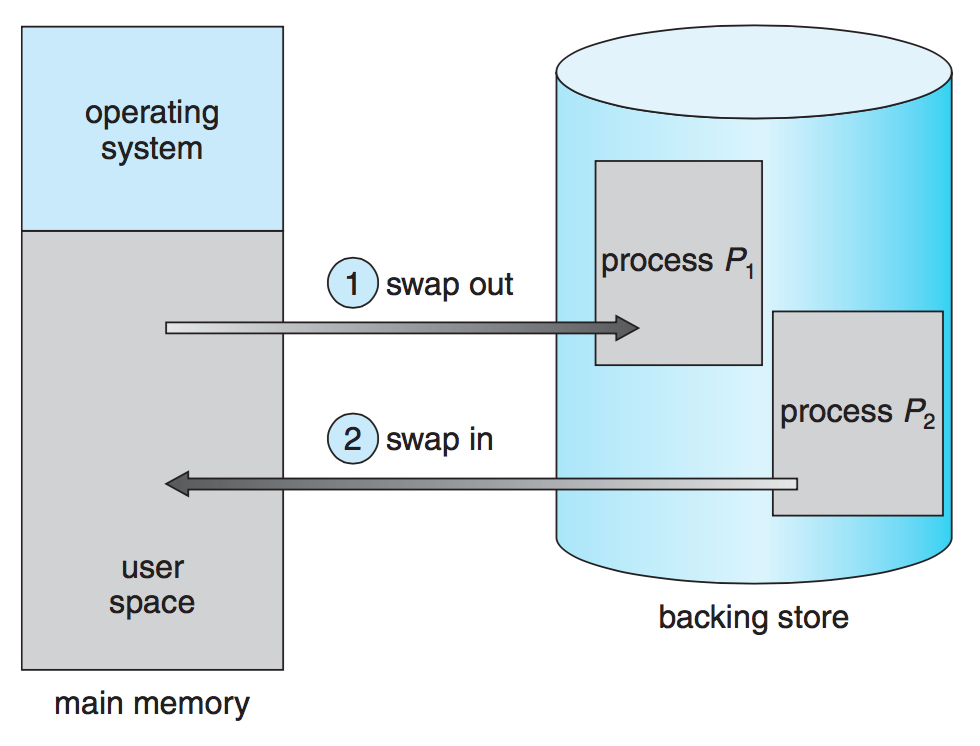
\includegraphics[width=0.75\textwidth]{images/swapping1.png}
\end{center}


\end{frame}

\begin{frame}
\frametitle{Swapping is Painful}

Unfortunately, swapping a process to disk is very painful. 

If the process is using 1~GB of memory, to swap a process out to disk, we need to write 1~GB of memory to disk. 

To load that process back later, it means reading another 1~GB from disk and putting it into main memory.
 
So, swapping is something we would like to do as little as possible.

\end{frame}

\begin{frame}
\frametitle{Swapping and Relocation}

When swapping a process back in from disk it is not necessary to put it back in exactly the same place as it originally was.

Just update the relocation register.

\begin{center}
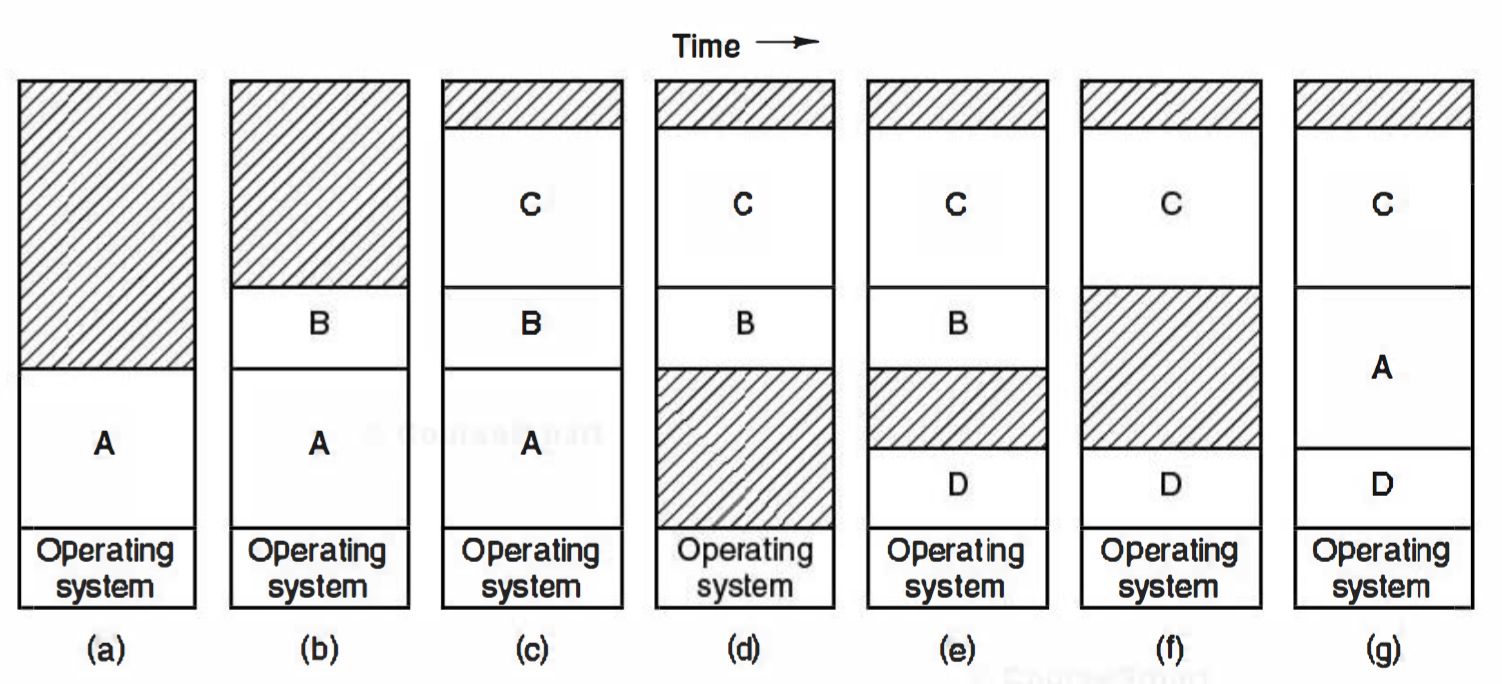
\includegraphics[width=0.8\textwidth]{images/swapping2.png}
\end{center}

\end{frame}

\begin{frame}
\frametitle{Memory Allocation}

Thus far we have considered process memory as a large, fixed-sized block.

 A process gets a big section of memory and operates in that area.
 
As you know from previous programming experience, use of the \texttt{new} keyword in some languages, or \texttt{malloc()} in C, will result in dynamic memory allocation. 

We will have to deal with this next...

\end{frame}
\end{document}

